%SI 2014-09-05

\documentclass{article}

\usepackage[T1]{fontenc}
\usepackage[utf8]{inputenc}
\usepackage[swedish]{babel}
\usepackage{fullpage}
\usepackage{amssymb}
\usepackage{bussproofs}
\usepackage{amsmath}
\usepackage{graphicx}
\usepackage{verbatim}
\usepackage{tikz}
\let\emptyset\varnothing


\title{Supplemental Instructions}
\author{Benjamin Eriksson \& Erik Thorsell \\ 
		\small{beneri@student.chalmers.se} \&
		\small{erithor@student.chalmers.se}
}
\date{
      %Place date here!
     }

\begin{document}
\maketitle


\subsection*{Vektorer}
\subsubsection*{1.}
Låt vektorerna $\vec{u} = (3,2)$, $\vec{v} = (0,1)$, $\vec{w} = (-2,2)$.
Rita linjärkombinationerna:
\begin{itemize}
\item[a) ] $\vec{u} + \vec{v}$  
\item[b) ] $2\vec{v} - \vec{w}$
\item[c) ] $\vec{u} + \vec{v} + \vec{w}$
\item[d) ] $-\vec{u} + (3\vec{v} - 2\vec{w})$
\end{itemize}



\subsubsection*{2.}
Skriv vektorerna $\vec{u}$, $\vec{v}$, $\vec{w}$ på koordinatform.

\noindent
\setlength{\unitlength}{0.75mm}
\begin{picture}(80,50)

\multiput(0,0)(5,0){17}%
{\line(0,1){45}}
\multiput(0,0)(0,5){10}%
{\line(1,0){80}}

\put(12,25){$\vec{v}$}
\put(16,5){$\vec{u}$}
\put(1,20){$\vec{w}$}
\thicklines
\put(10,10){\vector(1,2){10}}
\put(10,10){\vector(2,0){20}}
\put(10,10){\vector(-1,3){10}}
\end{picture}
\noindent
\newline
\newline

\noindent
Beräkna följande uppgifter:
\begin{itemize}
\item[a) ] $\vec{u} \cdot \vec{v}$  
\item[b) ] $\vec{v} \cdot \vec{w}$
\item[c) ] $||\vec{u}||$
\item[d) ] $||\vec{v}||$
\item[e) ] Beräkna vinkeln $\theta$ mellan  $\vec{u} $ och $ \vec{v}$ 
\end{itemize}

\subsubsection*{3.}
Låt vektorerna $\vec{u} = (2,2,5)$, $\vec{v} = (-2,3,1)$.
\begin{itemize}
\item[a) ] $||\vec{u} \times \vec{v}||$  
\item[b) ] $\vec{u} \times \vec{v}$
\item[c) ] $\vec{v} \times \vec{u}$
\item[d) ] Beräkna normalen till parallellogrammet som spänns upp av $\vec{u}$ och $\vec{v}$.
\item[e) ] Beräkna också arean till parallellogrammet.

\end{itemize}



\subsection*{Projektion och Spegling}
\subsubsection*{1.}
Låt $\vec{u} = (3,1)$ vara riktningsvektorn för linjen L och $\vec{v} = (3,2)$. 

\begin{itemize}
\item[a) ] Hitta den ortogonala projektionen, $\vec{v_L}$ av $\vec{v}$ på L.
\item[b) ] Hitta speglingen, $\vec{v_S}$ av $\vec{v}$ på L.
\end{itemize}

\noindent
\setlength{\unitlength}{0.75mm}
\begin{picture}(80,50)

\multiput(0,0)(5,0){17}%
{\line(0,1){45}}
\multiput(0,0)(0,5){10}%
{\line(1,0){80}}

\put(22,20){$\vec{v}$}
\put(27,11){$\vec{v_{L}}$}
\put(15,8){$\vec{u}$}
\put(60,30){$L$}
\thicklines
\put(10,10){\vector(3,2){30}}
\put(10,10){\vector(3,1){35}}
\put(10,10){\vector(3,1){10}}
\put(0,7){\line(3,1){70}}
\end{picture}
\noindent
\newline
\newline

\subsection*{Linjer och Plan}
\subsubsection*{1.}
Skriv ekvationen för linjen vilken passerar genom punkterna $A=(1,2)$ och 
$B=(2,5)$ på normal form, parameterform och {\it `` y=kx+m-form ''}.

\subsubsection*{2.}
Skriv ekvationen för linjen $r$ vilken passerar genom punkten $A=(1,5)$ och 
är parallell med den räta linjen $s$ mellan punkterna $(4,1)$ och $(-2,2)$.

\subsubsection*{3.}
Ett plan går genom punkterna $A=(1,1,-2)$, $B=(-1,5,2)$ och $C=(3,0,2)$.
Bestäm planets ekvation.\\


\clearpage
\subsection*{Lösningar}
\subsection*{Vektorer}
\subsubsection*{1.}
\begin{itemize}
\item[a) ] $(3,3)$  
\item[b) ] $(2,0)$  
\item[c) ] $(1,5)$  
\item[d) ] $(1,-3)$  
\end{itemize}
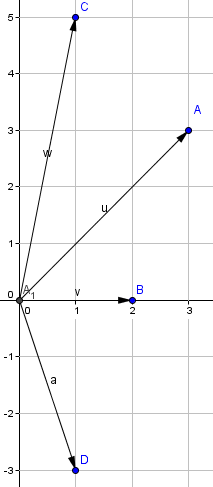
\includegraphics[scale=0.5]{graph_ans_1}



\subsubsection*{2.}
$\vec{u} = (4,0)$, $\vec{v} = (2,4)$, $\vec{w} = (-2,6)$.
\begin{itemize}
\item[a) ] $\vec{u} \cdot \vec{v} = 4*2 + 0*4 = 8$  
\item[b) ] $\vec{v} \cdot \vec{w} = 4*(-2) + 0*6 = -8$
\item[c) ] $||\vec{u}|| = \sqrt{4^2 + 0^2} = 4$
\item[d) ] $||\vec{v}|| = \sqrt{2^2 + 4^2} = \sqrt{20}$
\item[e) ] 
\[\vec{u} \cdot \vec{v} = ||\vec{u}|| \cdot ||\vec{v}|| \cdot cos \theta\]
\[cos \theta = \frac{\vec{u} \cdot \vec{v} }{ ||\vec{u}|| \cdot ||\vec{v}|| } \]
\[cos \theta = \frac{ 8 }{ 4 \sqrt{20} } \]
\[cos \theta \approx 63.4^{\circ} \]
\end{itemize}

\subsubsection*{3.}
\begin{itemize}
\item[a) ] $||(2 \cdot 1 - 5 \cdot 3, 5 \cdot (-2) - 2 \cdot 1, 2 \cdot 3 - 2 \cdot (-2))|| 
			= ||(-13, -12, 10)|| = \sqrt{413}$.
\item[b) ] $(-13, -12, 10)$
\item[c) ] $\vec{v} \times \vec{u} = -\vec{u} \times \vec{v} = (13, 12, -10)$
\item[d) ] Se b)
\item[e) ] Se a)
\end{itemize}

\subsection*{Projektion och Spegling}
\subsubsection*{1.}
$\vec{v_L} = (3.3, 1.1)$ och $\vec{v_S} = (3.6, 0.2)$. 
\[\vec{v_L} = \frac{\vec{u} \cdot \vec{v}}{\vec{u} \cdot \vec{u}}\vec{u}
= \frac{3*3+1*2}{3*3+1*1} (3,1) = \frac{11}{10} (3, 1) = (3.3, 1.1)\]. 

\[\vec{v_S} = 2\vec{v_L} - \vec{v} = (6.6, 2.2) - (3, 2) = (3.6, 0.2)\]
\newline  
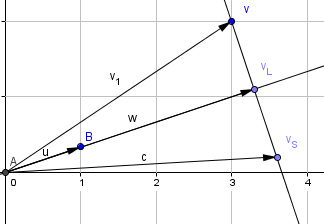
\includegraphics[scale=0.75]{graph_ans_3}

\subsection*{Linjer och Plan}
\subsubsection*{1.}
\begin{itemize}
\item[a) ]
{\bf Normal form: }
$x+y-3=0$
\item[b) ]
{\bf Slope-intercept form: }
$y=-x+3$
\item[c)]
{\bf Parameterform: }
$\left\{
\begin{array}{l l}
    x=1-3k\\
    y=2+3k
\end{array}\right.$
\end{itemize}

\noindent
\subsubsection*{2.}
$A=(1,5)$\\
$s \equiv 2x+y+2=0$ $\Leftrightarrow$ $y=-2x-2$

\noindent
Parallella linjer $\Rightarrow$ $k_{r} = k_{s} = \frac{-2}{1}$\\
Sätt in $x$ och $y$ från punkt $A$ $\Rightarrow$ $y-5 = -2(x-1)$ $\Rightarrow$ 
$2x+y-7=0$\\


\noindent
\subsubsection*{3.}
Normalen till planet ges av $\overrightarrow{n}=\overrightarrow{AB} \times 
\overrightarrow{AC} = (20,16,-6)$\\
Vi kan sedan använda punkten $A$ och vektorn $\overrightarrow{n_{2}}=
(10,8,-3)$ som är parallell med $\overrightarrow{n}$.\\
$A(x-x_{1})+B(y-y_{1})+C(z-z_{1})=0 \Rightarrow \\
10(x-1)+8(y-1)-3(z+2)=0 \Rightarrow \\
10x+8y-3z-24=0$

\end{document}
